\chapter{Fundamentação Teórica}

Nesse capítulo são apresentados os principais conceitos relacionados a proposta desse trabalho. Primeiramente são apresentados
os Sistemas de Recomendação e as suas abordagens tradicionais, seguidos pelos Sistemas de Recomendação Sensíveis ao Contexto
e os Sistemas de Recomendação Sensíveis ao Tempo. Em seguida são apresentadas as formas de avaliação de Sistema de Recomendação
e as formas de apresentação de Recomendações.

\section{Sistemas de Recomendação}

Sistemas de Recomendação (SRs) se tornaram uma importante área de pesquisa a partir dos anos 90, quando começaram a
surgir os primeiros trabalhos na área de filtragem colaborativa \cite{adomavicius2005toward}. Os SRs são ferramentas
computacionais que provém sugestões de itens personalizadas aos usuários \cite{ricci2011introduction}. Isso significa
que o usuário recebe como recomendação um conjunto diferente de itens de acordo com as suas preferências e necessidades.
Nos últimos anos, o interesse na aplicação de SRs têm crescido fortemente \cite{adomavicius2005toward, beel2016towards}.
Exemplos dessas aplicações são: recomendação de Livros, CDs, DVDs, etc., em sites de \textit{e-commerce} como Amazon e EBAY;
recomendações de filmes em sites como MovieLens e Netflix; recomendação de músicas em sites de \textit{streaming} como Last.fm ou
Spotify; recomendação de amigos ou de postagens em redes sociais como Facebook ou Twitter.

SRs estão representados formalmente na Equação \ref{eq:sr-tradicional}.

\begin{equation}
  F: U \times I \rightarrow R
  \label{eq:sr-tradicional}
\end{equation}

Onde $F$ é a função que busca prever o interesse do usuário pelos itens existentes, $U$ representa o conjunto dos usuários,
$I$ representa o conjunto dos itens e $R$ representa a lista ordenada dos itens pelo interesse previsto para o usuário ativo
(o usuário que irá receber a recomendação). O objetivo do SR então é conseguir prever de maneira mais correta, com as
informações disponíveis, os itens que serão de maior interesse do usuário.

Existem duas formas de capturar os interesses do usuário pelos itens acessados dentro do sistema: (1) Explicita, na
qual o usuário indica explicitamente o seu interesse pelo item que acabou de acessar, geralmente com uma nota 1 a 5 ou
apenas uma indicação de interesse positivo/negativo para o item; (2) Implícita, na qual o usuário não precisa indicar o
seu interesse pelo item, essa informação é capturada implicitamente através do seu comportamento e das suas interações
dentro do sistema.

Os SRs podem ser classificados de acordo com a forma como as recomendações são realizadas (abordagem). As principais
abordagens citadas na literatura são \cite{torres2004personalizaccao, adomavicius2005toward, ricci2011introduction}:
Baseada em Conteúdo, Filtragem Colaborativa, Baseada em Conhecimento e Híbrida. Nas subseções a seguir são descritas
cada uma dessas abordagens.

\subsection{Baseada em Conteúdo}\label{subsection:baseada-em-conteudo}

Segundo \citeonline{ricci2011introduction}, essa é uma abordagem na qual o usuário recebe recomendações de itens
similares aos que se interessou no passado. Consiste em avaliar a semelhança entre um item e os interesses do usuário.
Utilizando a nomenclatura utilizada por \citeonline{adomavicius2005toward}, os métodos dessa abordagem tentam prever o
grau de utilidade de um item para um usuário com base na utilidade que o usuário determinou para os itens similares ao item.

A abordagem Baseada em Conteúdo tem suas raízes na Recuperação da Informação \cite{adomavicius2005toward}. Para a
abordagem Baseada em Conteúdo, teremos um conjunto de atributos descrevendo um item e um conjunto de atributos
descrevendo os gostos e preferências do usuário. A descrição de um item frequentemente é realizada através de
palavras-chave definidas automaticamente por meio de algoritmos usados na área de Recuperação da Informação
\cite{adomavicius2005toward}. Já a descrição das preferências do usuário pode ser capturada de duas formas: implícita,
através do seu comportamento no ambiente e de itens que acessou; ou explícita, onde o usuário informa suas preferências
ao sistema, por exemplo, respondendo a questionários \cite{adomavicius2005toward}. Dessa forma, os SRs de itens
textuais (e.g., documentos) são os que mais utilizam a abordagem Baseada em Conteúdo, devido à facilidade da aplicação
das técnicas de Recuperação da Informação nesse tipo de item.

Dentro da área de Recuperação da Informação uma forma de medir a similaridade de itens em um SR é o Cosseno. O cálculo
da similaridade por Cosseno foi definido por Salton nos anos 60 \cite{salton1964document}. Nessa técnica, cada documento
é representado por um vetor de termos . Os vetores são dispostos em um espaço vetorial de  dimensões, onde  é o número
de termos, e documentos próximos nesse espaço são considerados semelhantes. Para verificar essa proximidade utiliza-se a
Equação \ref{eq:cosseno} \cite{christopher2008introduction}.

\begin{equation}
  sim(d_1, d_2) = \frac{\sum_{i=1}^{t}{w_{1,i} \times w_{2,i}}}{\sqrt{\sum_{i=1}^{t}{w_{1,i}}^2 \sum_{i=1}^{t}{w_{2,i}}^2}}
  \label{eq:cosseno}
\end{equation}


Onde: $sim(d_1, d_2)$ é o resultado da distância dos vetores, variando de $[0,1]$; $w_{1,i}$ é o termo presente na
posição $i$ do item $1$; $w_{2,i}$ é o termo presente na posição $i$ do item $2$. Por exemplo, se tivermos três vetores: $c = \{1,1\}$
representando o usuário, $v_1 = \{0, 1\}$ e $v_2 = \{1, 1\}$ representando itens. Ao calcular a similaridade entre esses itens,
temos $sim(c, v_1) \approx 0.71$ e $sim(c, v_2) = 1$, identificando que o item representado por $v_2$ é mais similar às
preferências do usuário $c$.

Outra técnica de Recuperação da Informação é o tf-idf (term-frequency inverse document frequency). Essa técnica
é utilizada para identificar termos importantes em um documento (MANNING et al., 2009) e pode ser utilizada
para a descoberta das palavras-chave que descrevem um item. É utilizada a fórmula da Equação \ref{eq:tf-idf} para o cálculo dos
pesos de cada termo do documento \cite{christopher2008introduction}.

\begin{equation}
  tf\hbox{-}idf_{t,d} = tf_{t,d} \times idf_{t,d}
  \label{eq:tf-idf}
\end{equation}

Onde: $tf\hbox{-}idf_{t,d}$ representa o peso do termo $t$ no documento $d$; $tf_{t,d}$ é o número de vezes que o termo
$t$ aparece no documento $d$; e $idf_{t,d}$ representa o Inverse Document Frequency do termo $t$, sendo o responsável por
identificar termos que aparecem em muitos documentos diferentes (MANNING et al., 2009). Os termos que aparecem em muitos
documentos tendem a perder sua importância. O $idf_{t,d}$ é calculado através da Equação \ref{eq:idf} \cite{christopher2008introduction}.

\begin{equation}
  idf_{t,d} = \log(\frac{N}{d_f})
  \label{eq:idf}
\end{equation}

Onde: $N$ é o número total de documentos em uma coleção; e $d_f$ é o número de documentos onde aparece o termo $t$.

A principal vantagem da abordagem Baseada em Conteúdo é não necessitar da opinião de outros usuários para a recomendação
\cite{ricci2011introduction}. As principais desvantagens são: o Cold-Start, em que o sistema não terá informações
suficientes sobre os usuários novos para realizar uma boa recomendação; e a Superespecialização, na qual o
usuário recebe sempre itens semelhantes aos que já viu \cite{lops2011content}.

\subsection{Filtragem Colaborativa}

Nessa abordagem o usuário receberá como recomendação itens que usuários com os mesmos interesses que ele se
interessaram no passado, ou seja, é a automatização do processo de "boca-a-boca" \cite{jannach2010recommender}. A
técnica de Filtragem Colaborativa tenta prever a utilidade  do item para o usuário, com base na utilidade do mesmo
produto para um conjunto de usuários  possuidores de características semelhantes às suas \cite{jannach2010recommender}.

Existem duas variações básicas da Filtragem Colaborativa: User-User, onde a similaridade entre os usuários é analisada;
Item-Item, onde a similaridade entre itens a serem recomendados é analisada \cite{jannach2010recommender}.

Para \citeonline{torres2004personalizaccao}, que considera a variação User-User, a Filtragem Colaborativa ocorre,
resumidamente, da seguinte forma:

\begin{enumerate}
\item As opiniões das pessoas sobre itens são armazenadas;
\item Baseado nessas opiniões, pessoas com perfil semelhantes (vizinhos) são agrupados;
\item Itens bem avaliados pelos vizinhos são recomendados ao usuário.
\end{enumerate}

Existem duas estratégias para medir a similaridade entre os usuários: Coeficiente de Pearson e Cosseno
\cite{torres2004personalizaccao}. Levando em consideração que os usuários são representados pelas notas que deram aos
itens, utiliza-se um cálculo matemático para medir a similaridade entre o perfil dos usuários
\cite{torres2004personalizaccao}.

O Coeficiente de Pearson é um coeficiente bastante utilizado em modelos econômicos e mede a força do relacionamento
de duas variáveis \cite{torres2004personalizaccao}. Esse coeficiente varia no intervalo $[-1, 1]$, sendo $-1$ indica
ausência de correlação e $+1$ indica forte correlação. O cálculo é então feito de acordo com a Equação \ref{eq:pearson}
\cite{torres2004personalizaccao}.

\begin{equation}
  w_{a,u} = \frac{\sum_{i=1}^{m}(r_{a,i} - \overline{r_a})*(r_{u,i} - \overline{r_u}))}{\sqrt{\sum_{i=1}^{m}(r_{a,i} - \overline{r_a})^2} \sqrt{\sum_{i=1}^{m}(r_{u,i} - \overline{r_u})^2}}
  \label{eq:pearson}
\end{equation}

Na fórmula, $w_{a,u}$ representa a correlação entre o usuário $u$ e um determinado usuário $a$, onde: $r_{a,i}$ é a avaliação
do usuário $a$ para o item $i$; $\overline{r_a}$ é a média de todas as avaliações do usuário $a$; $r_{u,i}$ é a avaliação do usuário
$u$ para o item $i$; $\overline{r_u}$ é a média de todas as avaliações do usuário $u$. A similaridade é calculada apenas com
itens que os dois usuários avaliaram.

Com o aumento da quantidade de usuários e de itens, se torna um desafio para a filtragem colaborativa User-User
realizar uma recomendação, principalmente pela dificuldade de identificar a vizinhança com tantos usuários
\cite{jannach2010recommender}. A estratégia Item-Item é uma solução para ser utilizada nesse contexto, permitindo a
computação das similaridades a acontecer off-line (JANNACH et al., 2011). A ideia principal da estratégia Item-Item
é prever a nota que o usuário daria para um item com base nas notas que ele deu para itens semelhantes àquele. Para
essa estratégia, o cálculo da similaridade pelo Cosseno, semelhante ao já citado, é uma métrica padrão e a que
apresenta os melhores resultados \cite{jannach2010recommender}. Esse cálculo da similaridade, ao invés de comparar
as notas de cada um dos usuários, considera vetores com as notas de cada item para identificar essa similaridade.

As pessoas que apresentaram preferências similares no passado tendem a concordar no futuro \cite{ricci2011introduction}.
Por isso essa abordagem tende a realizar recomendações que serão bem aceitas pelos usuários.

Como essa abordagem não considera a descrição dos itens e sim as notas desses, uma vantagem dessa abordagem é que as
recomendações realizadas podem ser bastante interessantes e inesperadas ao usuário \cite{ricci2011introduction}.

Por outro lado, a abordagem colaborativa também possui a desvantagem de Cold-Start. Existem dois tipos de Cold-Start
nessa abordagem \cite{adomavicius2005toward}: o User Cold-Start e o Item Cold-Start. O User Cold-Start é a dificuldade
que o sistema encontra para recomendar um item para um usuário que não avaliou nenhum item ainda. O Item Cold-Start
ocorre para um novo item no sistema, que não será recomendado enquanto não for avaliado por algum usuário.

Além disso, outras desvantagens são \cite{adomavicius2005toward}:

\begin{itemize}
\item Esparsidade: quanto maior a quantidade de usuários e de itens disponíveis, mais esparsa ficará a tabela com as
notas dos usuários e mais difícil será realizar as comparações. Pode ser difícil prever com precisão usuários com os
mesmos gostos, pois cada usuário poderá avaliar conjuntos muito diferentes de itens;
\item Necessidade de uma comunidade de usuários ativa: para essa abordagem é necessário ter uma grande quantidade de
usuários ativas no sistema ao mesmo. No caso de um sistema com poucos usuários pode acontecer também a esparsidade
pois os usuários acessaram e avaliaram itens diferentes e  não possível calcular a similaridade entre eles;
\item Ovelha Negra: para usuários que possuem gostos distintos demais, se torna um desafio realizar recomendações
interessantes para ele. O principal motivo é que não conseguiremos definir outros usuários semelhantes a ele para comparar;
\item Escalabilidade: com o aumento do número de usuários, o custo computacional se torna alto;
\item Confiabilidade: esse problema se refere à confiabilidade das avaliações realizadas pelos usuários, se forem
realizadas de forma incorreta irão diminuir a eficiência da abordagem. Outra coisa a ser considerada é a reputação dos
usuários: usuários com maior reputação poderiam ter suas avaliações mais consideradas (maior peso) que as outras de
outros usuários.
\end{itemize}

\subsection{Baseada em Conhecimento}

A abordagem Baseada em Conhecimento recomenda itens aos usuários com base no conhecimento que o sistema possui sobre
como características de um item se encaixam nas necessidades de um usuário e o quão útil esse item será
\cite{ricci2011introduction}. O sistema recebe como entrada a descrição das necessidades e interesses do usuário e o
papel do sistema é realizar uma combinação entre essas necessidades e os itens.

Os SRs Baseado em Caso (Case-Based) são um exemplo de SR da abordagem Baseada em Conhecimento. Nesse sistema uma
função de similaridade estima o quanto a necessidade de um usuário (descrição de um problema) combina com uma
determinada recomendação (solução do problema) \cite{ricci2011introduction}. Essa similaridade é o grau de utilidade
da recomendação.

Outro exemplo da abordagem Baseada em Conhecimento são os SR Baseados em Restrição. Nessa abordagem os itens que não
atendam a certas restrições são automaticamente eliminados dos itens a serem recomendados. Segundo
\citeonline{ricci2011introduction}, a principal diferença entre um SR Baseado em Caso e um Baseado em Restrição está
no fato de o Baseado em Caso considerar a similaridade entre as necessidades do usuário e o item enquanto a baseada
em restrições possui regras específicas para tratar cada uma das necessidades do usuário.

A abordagem Baseada em Conhecimento costuma funcionar melhor que outras (e.g., Filtragem Colaborativa ou Baseada em
Conteúdo) no início do desenvolvimento, porém se ela não for equipada com a capacidade de aprender mais sobre o usuário,
ela será rapidamente ultrapassada por métodos mais simples que exploram a interação do usuário com o sistema
\cite{ricci2011introduction}.

\subsection{Híbrida}

Essa abordagem utiliza uma combinação das diversas abordagens para recomendar itens ao usuário. O objetivo é reunir as
vantagens das abordagens e tentar eliminar suas desvantagens \cite{burke2002hybrid}. As principais abordagens que são
combinadas são a Baseada em Conteúdo e Filtragem Colaborativa, por serem as mais tradicionais e mais utilizadas
\cite{adomavicius2005toward}. Alguns exemplos de algoritmos que utilizam a abordagem híbrida foram dados por
\citeonline{burke2002hybrid}:

\begin{itemize}
\item Weighted: a recomendação é o resultado da execução das duas abordagens de recomendação. Essas abordagens podem
ser executadas linearmente, uma após a outra, para definir os melhores itens a serem recomendados, ou cada abordagem
pode ter pesos diferentes, tornando o resultado de um mais importante que o resultado do outro.
\item Switching: ocorre uma alternância entre as duas abordagens, em certos momentos uma delas é utilizada e em outros
momentos a outra é utilizada. O sistema deverá possuir alguns critérios para definir qual abordagem irá utilizar.
\item Mixed: as duas abordagens mencionadas são utilizadas e os resultados aparecem em um mesmo ranking. Esse tipo de
abordagem é utilizado quando se deseja realizar um grande número de recomendações diferentes simultaneamente.
\item Feature combination: considera as informações da colaboração como uma característica e utiliza a abordagem
Baseada em Conteúdo para realizar a recomendação.
\item Cascade: uma abordagem é utilizada primeiro para gerar um ranking e a outra abordagem refina o resultado dado
por esta.
\item Feature augmentation: uma abordagem é utiliza para produzir um ranking ou uma classificação para cada item e o
resultado será considerado na execução da outra abordagem.
\end{itemize}

\section{Sistemas de Recomendação Sensíveis ao Contexto}\label{section:sr-sensivel-contexto}

SRs tradicionais consideram apenas as relações entre os usuários e os itens para recomendar, mas não consideram o
contexto em que os usuários estão. De acordo com \citeonline{dey2001understanding}, o contexto é qualquer informação
que pode ser usada para caracterizar a situação de uma entidade. Sendo as principais entidades em SRs o usuário que
irá receber uma recomendação e os itens que serão recomendados.

SRs Sensíveis ao Contexto estão formalmente definidos na Equação \ref{eq:context-aware}.

\begin{equation}
  F: U \times I \times C \rightarrow R
  \label{eq:context-aware}
\end{equation}

Onde $F$ é a função que prediz o interesse em um item ainda não utilizado pelo usuário, $U$ representa o conjunto do
usuários, $I$ representa o o conjunto dos itens, $C$ representa o contexto da interação e $R$ representa o conjunto de itens
ordenado pelo interesse previsto do usuário para os itens disponíveis.

Vários autores definem conjuntos de dimensões que podem representar o contexto
\cite{schilit1994context, chen2000survey, zimmermann2007operational} e que diferem pouco entre si. Nesse trabalho,
nós seguimos a definição de \citeonline{schmidt1999there}, que é uma das mais completas encontradas:

\begin{itemize}
\item Informações sobre o usuário, e.g., hábitos do usuário, estado emocional, etc.;
\item Ambiente social do usuário, e.g., co-localização com outros usuários, interação em redes sociais, etc.;
\item Tarefas do usuários, e.g., objetivos gerais, se é uma tarefa definida previamente (pelo professor, por exemplo)
ou aleatória, etc.;
\item Localização, e.g., posição absoluta, se o usuário está em casa, no trabalho ou na universidade, etc.;
\item Condições do ambiente, e.g., barulho, luminosidade, etc.;
\item Infraestrutura, e.g., velocidade da internet, tipo de dispositivo utilizado, etc.;
\item Tempo, e.g., \textit{timestamp} de ocorrência de uma interação, dia da semana no qual o usuário pede uma recomendação, etc.
\end{itemize}

\citeonline{adomavicius2011context} definem três paradigmas de uso das dimensões do contexto no processo de recomendação:

\begin{itemize}
\item Pré-Filtragem Contextual, na qual o contexto filtra os dados que representam o usuário e esses dados servem
como entrada para um algoritmo tradicional de recomendação;
\item Pós-Filtragem Contextual, na qual uma abordagem tradicional de recomendação é utilizada para gerar uma lista de
itens a ser recomendados e depois esses itens são filtrados de acordo com o contexto do usuário;
\item Modelagem Contextual, na qual o contexto é aplicado diretamente no algoritmo de recomendação, gerando um
algoritmo diferente dos tradicionais.
\end{itemize}

\citeonline{verbert2012context} dizem que, em ambientes educacionais, as abordagens tradicionais de SRs não são
suficientes para recomendar de forma apropriada para os estudantes, porque esse domínio oferece algumas características
específicas que não são cobertas por essas abordagens. Por exemplo, é muito mais perigoso recomendar um item ruim para
um estudante, que pode desmotiva-lo nos seus estudos, do que recomendar um produto ruim em um site de \textit{e-commerce}.
De acordo com \citeonline{verbert2012context} esse domínio requer um nível maior de personalização.

Aplicar algumas dimensões do contexto é uma alternativa para melhorar a personalização em ambientes educacionais,
recomendando materiais adequados para a situação atual do usuário. Por exemplo, considerar o histórico de aprendizagem
do aluno, as condições do ambiente e a acessibilidade dos recursos \cite{verbert2012context}.

Na próxima seção é apresentado um tipo específico de SRs Sensíveis ao Contexto que utilizam a dimensão temporal para
recomendar. Esse tipo de SR pode também aplicar outras dimensões do contexto em conjunto.

\section{Sistemas de Recomendação Sensível ao Tempo}\label{section:sr-sensivel-tempo}

Dentre as dimensões do contexto citadas na seção \ref{section:sr-sensivel-contexto}, o tempo tem uma vantagem de ser
fácil de capturar, considerando que praticamente todos os dispositivos tem um relógio que pode capturar o tempo no qual
alguma interação ocorreu. Além disso, trabalhos na área demonstraram que o contexto temporal tem potencial para melhorar
a qualidade das recomendações \cite{campos2014time}. Esse tipo de SR é chamado de SR Sensível ao Tempo.

SRs Sensíveis ao Tempo estão formalmente definidos na Equação \ref{eq:time-aware}.

\begin{equation}
  F: U \times I \times T \rightarrow R
  \label{eq:time-aware}
\end{equation}

Onde F é a função que prediz o interesse do usuário por item ainda não utilizado, U representa o conjunto de usuários,
I representa o conjunto de itens, T representa o contexto temporal e R representa o conjunto de itens ordenado pelo interesse previsto do usuário para os itens disponíveis.

De acordo com o dicionario \citeonline{michaelis2011disponivel}, o tempo é um  "Período de momentos, de horas, de dias,
de semanas, de meses, de anos etc. no qual os eventos se sucedem, dando-se a noção de presente, passado e futuro".
Com essa informação é possível para um sistema computacional estabelecer uma ordem para os eventos que ocorrem.

O Tempo pode ser representado de uma variável contínua ou categórica. A representação contínua utiliza o exato momento
em que os itens foram consumidos/avaliados \cite{campos2014time}, por exemplo: "8 de outubro de 2017, 16:15:03".
Enquanto na representação categórica as variáveis são calculadas relação a períodos de interesse \cite{campos2014time},
e.g., Dias da semana: {Domingo, Segunda, Terça, ...} ou Estações do ano: {Primavera, Verão, Outono, Inverno}. Além
disso, o tempo pode ser representado por diferentes unidades de tempo, e.g., segundos, minutos, horas, meses, anos,
etc., e as unidades tempo são hierárquicas, e.g., um dia tem 24 horas, uma hora tem 60 minutos e 1 minuto tem 60
segundos.

Um mapeamento sistemático foi conduzido sobre os SR Sensíveis ao Tempo \cite{de2017time} utilizando a metolodolia de
\citeonline{petersen2008systematic}. Nesse mapeamento sistemático não foi restringido apenas trabalhos na área
educacional. A principal questão de pesquisa desse mapeamento foi: Como o contexto temporal é utilizado em SRs
Sensíveis ao Contexto? Para responder a essa questão de pesquisa principal, três questões de pesquisa secundárias
foram definas, são elas: (1) Como os algoritmos de recomendação utilizam o tempo? (2) Qual é a diferença entre o uso
do tempo em diferentes domínios de aplicação? (3) Que outras dimensões são utilizadas juntamente com o contexto
temporal?

Após o processo de seleção dos artigos, 88 trabalhos fizeram parte do estudo e foram considerados para responder as
questões de pesquisa. Entre os resultados do mapeamento sistemático desenvolvido em \citeonline{de2017time}, o principal
foi a definição de sete categorias de SRs Sensíveis ao Tempo. Essa categorização foi feita a partir do agrupamento
dos artigos que utilizam o tempo de forma semelhante. A partir disso foi possível identificar as sete principais
formas de utilizar o tempo nos algoritmos de recomendação que são descritas nas próximas subseções.

\subsection{Restriction}

Na categoria Restriction, o tempo é utilizado para restringir que itens serão utilizados. Isso significa que o SR
compara variáveis de tempo relacionadas aos itens e ao usuário para restringir quais itens irão aparecer na lista de
recomendações. Existe pelo menos duas formas de restrição para se utilizar: (1) o SR compara o tempo disponível pelo
usuário com o tempo necessário para consumir um determinado item, e.g., a duração dos filmes que serão recomendados e
o tempo que o usuário tem até o seu próximo compromisso; (2) o SR compara o tempo atual (data e hora) com o horário de
funcionamento dos itens que serão recomendados, e.g., na recomendação de restaurantes onde só faz sentido recomendar
locais que estejam servindo no momento.

\subsection{Micro-profile}

Na categoria Micro-Profile, o usuário possui perfis distintos para cada período de tempo. Nessa categoria, o tempo
deve ser utilizado de forma categórica, onde as categorias que serão utilizadas dependem da aplicação onde for aplicada.
É possível, por exemplo, que o usuário possua um perfil para dias da semana e outro perfil para finais de semana, ou
então um perfil para a manhã, outro para a tarde e outro para a noite. O objetivo é que as recomendações serão
realizadas considerando apenas as interações do usuário que aconteceram no mesmo contexto temporal em que ele está no
momento, e.g., recomendar programas de TV para o usuário em um domingo a noite considerando apenas quais programas ele
costuma acessar em um domingo a noite.

\subsection{Bias}

Na categoria Bias, o tempo é utilizado para agregar informação na matriz Usuários x Itens normalmente utllizada pela
Filtragem Colaborativa. Essa matriz é comumente utilizada com apenas duas dimensões que são os Usuários e o Itens e os
valores dessa matriz são as notas dadas pelos usuários para os itens. Ao incorporar o tempo nessa matriz, é possível
realizar uma comparação mais precisa entre os usuários do sistema e assim prever o interesse do usuário ativo para os
itens ainda não acessados. Dessa forma, usuários que avaliaram os mesmos itens com notas semelhantes e em contextos
temporais semelhantes serão considerados vizinhos do usuário ativo e o algoritmo de recomendação tem uma maior chance
de acertar nos interesses do usuário.

\subsection{Decay}\label{section:decay}

Na categoria \textit{Decay}, o tempo é utilizado como um fator de decaimento na importância das interações do usuário, i.e.,
interações (itens consumidos, avaliações, etc.) mais antigas tem um peso menor para o algoritmo de recomendação do que
as interações mais atuais. Os algoritmos dessa categoria consideram que o interesse do usuário varia com o tempo e é
importante considerar que os interesses mais atuais do usuário representam melhor o seu perfil do que interesses mais
antigos. É importante notar que as interações antigas não são ignoradas pelo algoritmo de recomendação com \textit{Decay}, é
apenas dado um peso menor para essas interações.

\subsection{Time Rating}

Na categoria \textit{Time Rating}, o tempo é considerado pelo SR para inferir as preferências do usuário. Nessa categoria o SR
utiliza uma estratégia implícita para capturar o interesse do usuário que considera o tempo que o usuário passou em
determinado item. A categoria toma como princípio que itens no qual o usuário passou pouco tempo não são do seu
interesse, enquanto itens em que ele passou mais tempo indicam os seus interesses. Essa forma de capturar é interessante
pois o usuário não precisa explicitamente dar notas ao itens, dessa forma é possível capturar um feedback do usuário
para todos os itens acessados por ele.

\subsection{Novelty}

Na categoria \textit{Novelty}, o SR considera que itens mais novos serão mais relavantes para os usuários do que itens mais
antigos. Nessa catoria, existem pelo menos duas estratégias que podem ser utilizadas: (1) o SR possui uma idade limite
definida (por exemplo, duas semanas) e itens que sejam mais velhos que isso serão retirados da lista de recomendação;
(2) o SR não ignora itens antigos, porém os itens novos possuem um peso maior e, se dois itens similares estiver para
ser recomendados, o mais novo é o escolhido mesmo que o mais antigo esteja mais de acordo com o perfil do usuário.
Essa categoria é mais comum em domínios onde novos itens tendem a ser mais relevantes que itens antigos, e.g., redes
sociais, notícias, etc.

\subsection{Sequence}

Na categoria \textit{Sequence}, o SR observa itens que são geralmente consumidos juntos em uma determinada ordem e utiliza essa
informação para recomendar. Dessa forma, quando o SR encontra um padrão nos acessos de um usuário que já é conhecido,
é possível utilizar os próximos itens da sequência como recomendações para o usuário. Essa categoria que os usuários
tendem a seguir algum padrão de acesso (trajetória) enquanto interagem com o sistema.

\section{Avaliação de Sistemas de Recomendação}

A avaliação de SR são divididas em três categorias \cite{shani2011evaluating}:

\begin{itemize}
\item Experimentos \textit{offline}, avaliação do método de recomendação através de uma base de dados, simulando as ações
dos usuários sem necessitar da participação dos mesmos;
\item Estudos com os usuários, em que um pequeno grupo de usuários realiza tarefas específicas relacionadas ao SR e
podem ser utilizados em conjunto com medidas qualitativas para mensurar a satisfação dos usuários, por exemplo através
de questionários;
\item Uso real do sistema, na qual o SR é avaliado em situações reais de uso e os dados para avaliação quantitativa são
capturados de forma automática, por exemplo ferramentas de \textit{Web Analytics}.
\end{itemize}

\citeonline{pu2011user} propõe um framework para a avaliação de SRs utilizando \textbf{Estudos com os usuários}, com o objetivo
de realizar uma avaliação do SR através da Experiência do Usuário. Esse \textit{framework} se chama \textit{Recommender
Systems' Quality of User Experiente}  (ResQue) e foi proposto com base em outras ferramentas para avaliação centrada no
usuário não exclusivas de SR: \textit{Technology Acceptance Model} (TAM), que define três construtos FFacilidade de Uso
Percebida), Utilidade Percebida e Intenções do Usuário em utilizar o sistema e \textit{Software Usability Measurement
Inventory} (SUMI), que consiste de cinco construtos (Eficiência, Influência, Ajuda, Controle, Capacidade de Aprendizado)
e um questionário de 50 questões.

O \textit{framework} proposto por \citeonline{pu2011user} consiste em quatro construtos: (1) Qualidades Percebidas pelos
Usuários, (2) Crenças/Opiniões do Usuário, (3) Atitudes/Propósitos do Usuário, (4) Intenções Comportamentais.
Para cada um dos construtos, vários aspectos são avaliados, como pode ser visto na Figura \ref{fig:resque-framework}.
Os autores definem ainda um conjunto de 60 questões para aplicar nessa avaliação como pode ser visto no Anexo
\ref{ane:questoes-framework}. Nesse questionário as questões são afirmações nas quais o usuário deve ser posicionar em
um escala de Likert de 5 pontos, de "Discordo totalmente" até "Concordo totalmente". Os autores ainda afirmam que o
conjunto de questões aplicado pode ser reduzido para um subconjunto com 15 questões (questões com asterisco no Anexo
\ref{ane:questoes-framework}).

\begin{figure}[htb]
  \caption{\label{fig:resque-framework}Construtos do framework de avaliação de SRs centrado no usuário}
  \begin{center}
      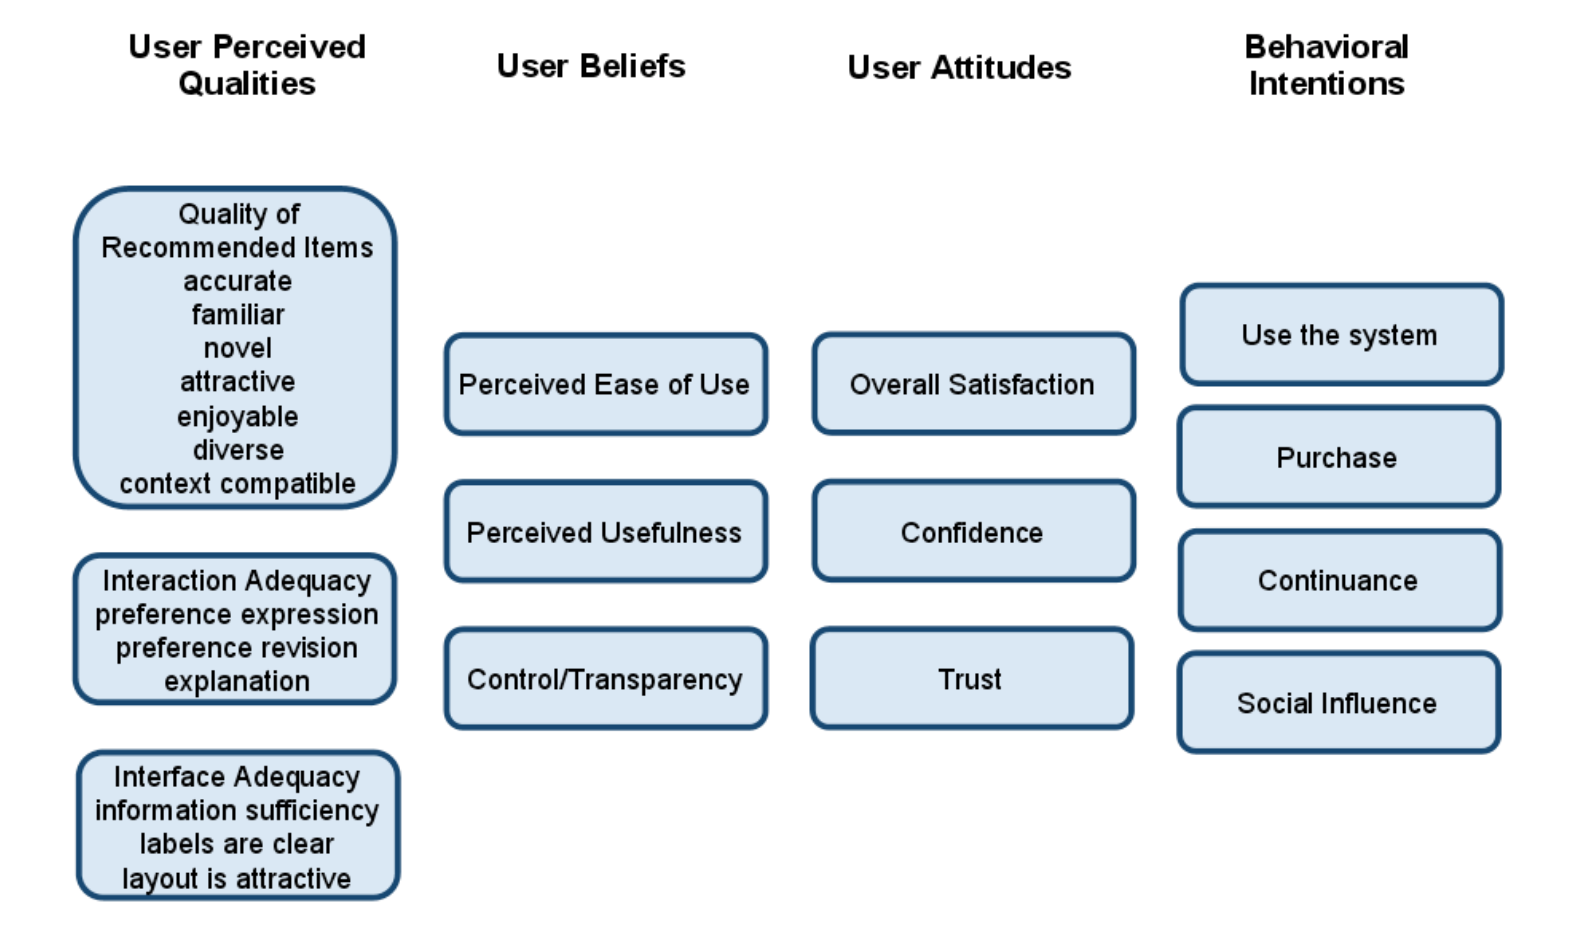
\includegraphics[scale=0.6]{./Figuras/resque-framework.png}
  \end{center}
  \legend{Fonte: \citeonline{pu2011user}}
\end{figure}

\section{Apresentação das Recomendações}\label{section:fundamentacao-apresentacao-recomendacao}

No trabalho de \citeonline{pu2012evaluating} os autores argumentam que apenas a eficiência do algoritmo não garante
que o usuário estará satisfeito com o sistema, será leal e continuará utilizando-o ou que os itens serão "convertidos"
(nesse sentido, os autores se referem a conversão como a aceitar a recomendação dada e utilizar/comprar/assistir/etc.
o item recomendado). Os autores afirmam que percepção do usuário sobre a qualidade da recomendação é afetada tanto pela
qualidade das recomendações, que é responsabilidade do algoritmo de recomendação, quanto pela eficiência na apresentação
das recomendações, explicando a razão daquelas recomendações e inspirando a confiança do usuário nas suas decisões.
Para isso, os autores defendem uma avalição do SR centrada no usuário, de forma a avaliar não somente o algoritmo de
recomendação mas o SR como um todo \cite{pu2012evaluating}.

Além disso, \citeonline{pu2012evaluating} definem um conjunto de vinte diretrizes para o design de um SR bem aceito
pelos usuários. Essas diretrizes foram criadas a partir da combinação do resultado de vários trabalhos que executaram
experimentos com participação de usuários (i.e., Estudos com usuários) para avaliar a interface de SRs. As principais
diretrizes levadas em conta por esse trabalho são \cite{pu2012evaluating}:

\begin{itemize}
\item Diretriz 14: Considere aprimorar a acurácia percebida pelo usuário com um \textit{layout} mais atrativo, rótulos mais
efetivos, e explicando como o sistema gerou as recomendações. Fazendo isso pode aumentar a percepção do usuário sobre a
eficiência do sistema, sua satisfação com o sistema em geral, sua prontidão para aceitar os itens recomendados e a sua
confiança no sistema.
\item Diretriz 18: Considere fornecer como recomendação itens compatíveis ao contexto do usuário. Essa característica
pode estar altamente relacionada com a percepção de utilidade do sistema e da satisfação do usuário.
\item Diretriz 19: Considere explicar porque o sistema recomendou determinados itens. Esses aspectos podem estar
altamente relacionados com a satisfação do usuário, a percepção de controle, as intenções do usuário inspiradas pela
confiança do usuário, como a intenção de retornar ao sistema.
\item Diretriz 20: Considere fornecer informação suficiente relacionadas aos itens recomendados, controlar a qualidade
das informações e da estrutura de navegação.
\end{itemize}

\section{Considerações sobre o capítulo}

Nesse capítulo foram apresentados os principais conceitos relacionados a Sistemas de Recomendação (SRs) Sensíveis ao Tempo.
Foram apresentadas desde as abordagens tradicionais, passando pelos SR Sensíveis Contexto e os seus paradigmas até as
categorias de SRs Sensíveis ao Tempo definidas em \citeonline{de2017time}.

Dentre as categorias de SRs Sensíveis ao Tempo apresentadas na Seção \ref{section:sr-sensivel-tempo}, a utilizada por esse
trabalho é o \textit{Decay}. Nessa categoria é considerado que o interesse do usuário por um item acessado diminui com o passar
do tempo. Para isso, itens acessados recentemente tem um peso maior no algoritmo de recomendação e os itens vão perdendo
o peso gradativamente.

Além disso, foi apresentada as formas de avaliação de um SR como definido por \citeonline{shani2011evaluating}. Neste
trabalho é utilizada uma avaliação centrada no usuário, como orientado por \citeonline{pu2012evaluating}. Por isso, é
apresentado o \textit{framework} definido por \citeonline{pu2011user} que busca avaliar a experiência do usuário através de um
questionário com 60 questões dividas nos quatro construtos do \textit{framework}. Para ser utilizado, será necessário
selecionar quais das questões serão utilizadas, pois como citado por \citeonline{pu2011user} nem todas as questões se
aplicam a todos os SRs, e traduzir essas questões para tornar possível a aplicação.

Na Seção \ref{section:fundamentacao-apresentacao-recomendacao} são apresentados algumas diretrizes definidas por
\citeonline{pu2012evaluating} para a apresentação das recomendações. Essas diretrizes foram definidas através de
experimentos com participação do usuário e serão consideradas para a definição da interface da proposta desse trabalho.
